\clearpage
\section{Materials Informatics and Compositional Similarity}

Materials informatics (MI), and in particular Quantitative Structure--Property Relationship
(QSPR) modeling, is a key tool in modern materials discovery. Its main idea is simple:
\textbf{materials with similar compositions and chemistry often have similar physical
properties}. This directly relates to our challenge of predicting whether a material is
stable, magnetic or metallic using limited computed data (Section~1).

MI represents every material as a numerical vector called a \textbf{descriptor} vector. For a
chemical formula, the most widely used descriptors are the \emph{Magpie} statistics: for 22
elemental properties (electronegativity, covalent radius, number of valence electrons,
melting temperature, elemental band gap, magnetic moment, \dots) we compute the
composition-weighted minimum, maximum, range, mean, average deviation and mode. Models trained
on materials with known properties can then predict the properties of new compositions in
milliseconds, which is particularly useful when labeled data is scarce and the pool of
untested candidates is huge.

A typical MI workflow includes:

\begin{enumerate}
  \item Collecting a dataset of materials with known properties.
  \item Calculating composition (or structure) descriptors.
  \item Selecting the most relevant descriptors to avoid overfitting.
  \item Building predictive models using regression or classification methods.
  \item Validating models with cross-validation and external test sets.
\end{enumerate}

MI not only predicts properties but also highlights which chemical features matter, guiding
the design of better materials. It also reduces reliance on expensive DFT calculations and
laboratory synthesis.

\begin{figure}[H]
  \centering
  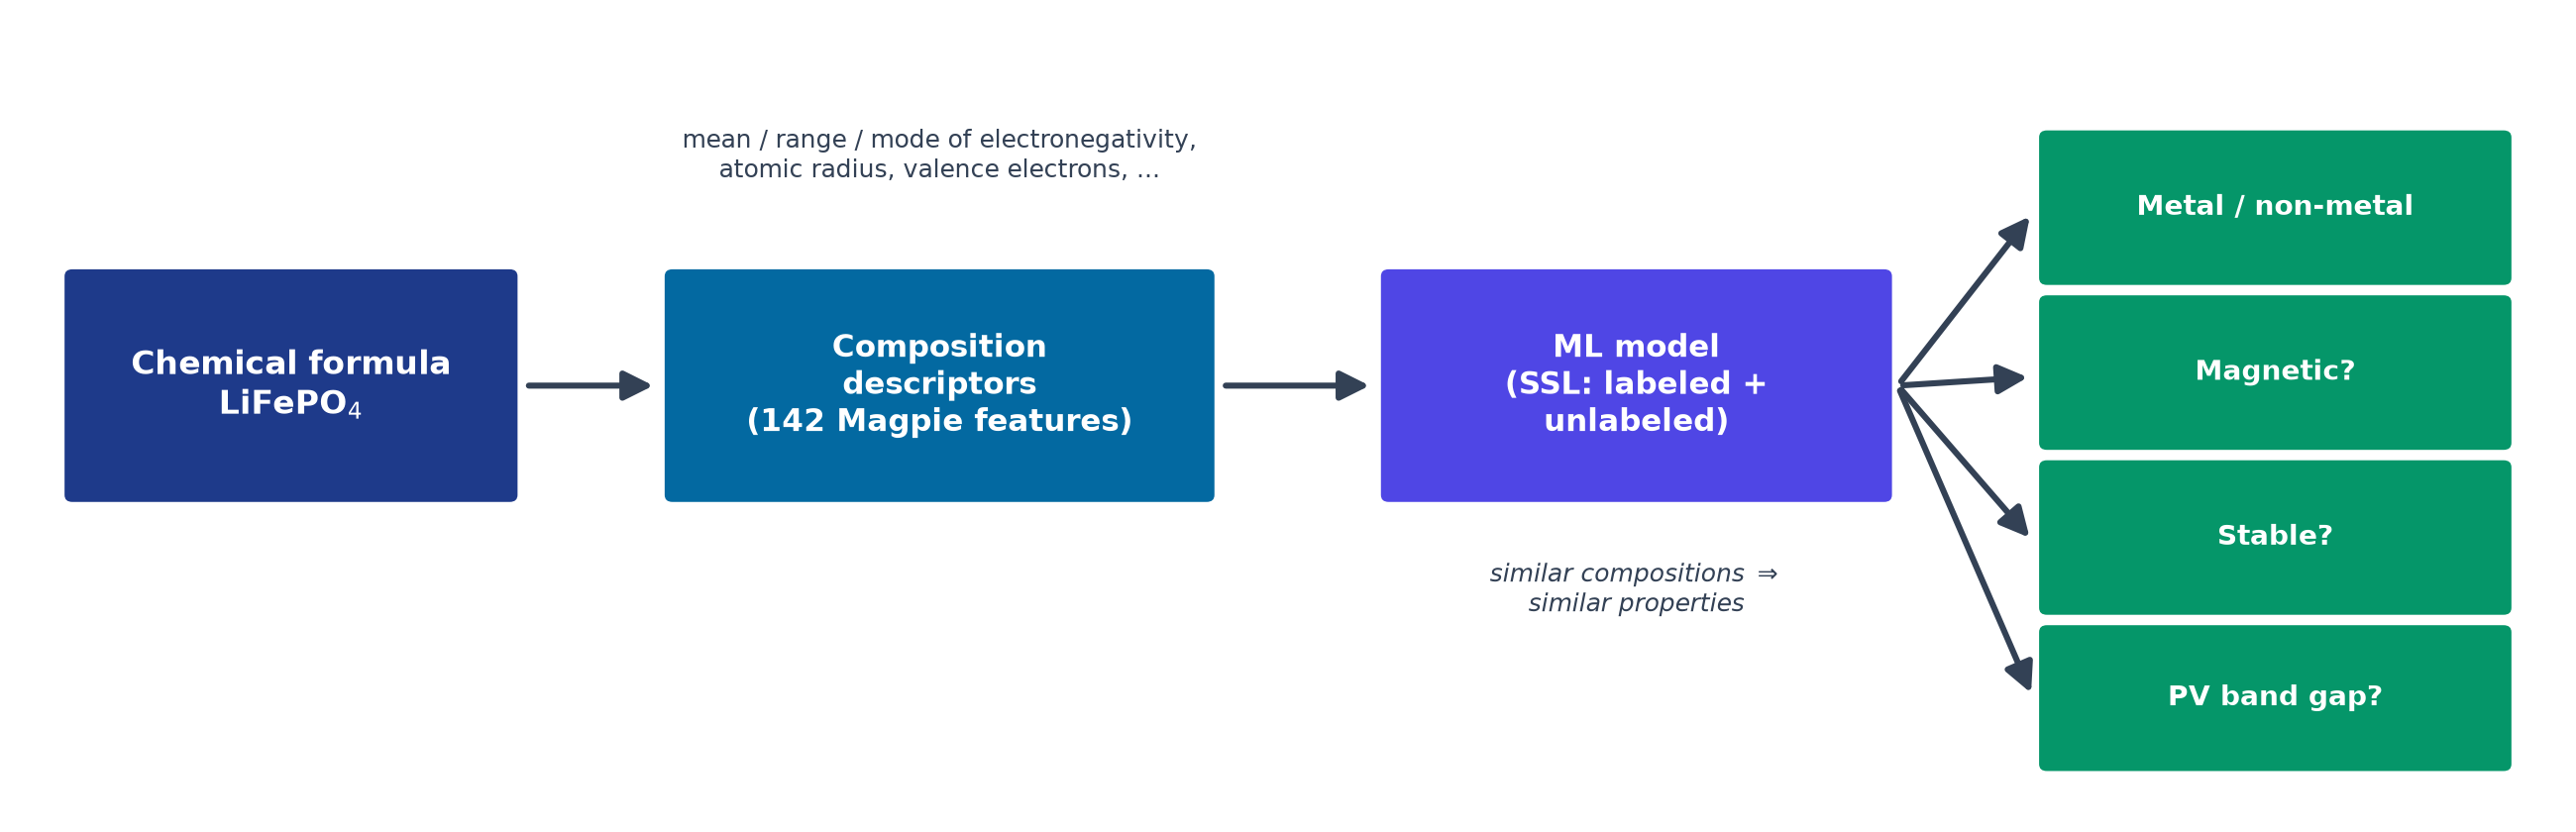
\includegraphics[width=\textwidth]{schematics/mi_principle.png}
  \caption{Materials-informatics principle}
\end{figure}

Building on MI, Semi-Supervised Learning (SSL) can further improve predictions by
incorporating the large pool of unlabeled compositions. Combining MI with SSL allows models to
learn from both labeled and unlabeled data, addressing the challenges of property prediction
and data scarcity.
